\documentclass[12pt]{article}
\usepackage[a4paper, margin=.30in]{geometry}
\usepackage{graphicx ,
            wrapfig,
            xcolor, 
            enumerate,
            amsmath,fontenc, mhchem,makecell, mhchem,tcolorbox,tikz,fancyhdr
            }

\newcommand\headerMe[2]{\noindent{}#1\hfill#2}
\renewcommand{\thesection}{\Roman{section}}
\author{Zakaria HAOUZAN}
\date{\today}

\definecolor{copper}{cmyk}{0,0.9,0.9,0.2}
\colorlet{lightgray}{black!25}
\colorlet{darkgray}{black!75}

\pagestyle{fancy}
\fancyhf{}
\rhead{2022/2023}
\lhead{Pr: Zakaria HAOUZAN}
\chead{Physique Chimie}
\rfoot{lycée :  skhor rhamna}
\cfoot {Page \thepage}


\begin{document}
% headers --------------
\headerMe{Matière : Physique-Chimie}{Professeur : Zakaria HAOUZAN}\\
\headerMe{Unité :Sens d'évolution d'un système chimique  }{Établissement : Lycée SKHOR qualifiant}\\
\headerMe{Niveau : 2BAC-SM-PC}{Heure : 6H}\\

% ------Content ________


\begin{center}

    \Large{Leçon $N^{\circ} 10 $: \color{red} Transformations forcées - L'électrolyse }
\end{center}
\section{Transformation Spontanées dans une pile :}
\subsection{Transformation spontanée entre le cuivre métal et le dibrome en solution aqueuse : }
On mélange dans un tube à essaie la tornure de cuivre $(Cu_{(s)})$ et une solution de dibrome $Br_{2(aq)}$ de concentration $10^{-2}mol/L$.

La solution initiale est rouge-orange (couleur du dibrome en solution).

On constate: 
\begin{itemize}
	\item la disparition de la coloration du dibrome $Br_{2(aq)}$.
	\item la dispatition du métal cuivre .
	\item la solution se colore progressivement en bleu ( cette coloration est due à l'apparition des ions $Cu^{2+}$).

	\item Une réaction d’oxydo-réduction s’est produite spontanément entre $Cu_{(s)}$ et $Br_{2(aq)}$ avec formation des ions $Cu^{2+}_{(aq)}$ et $Br^-_{(aq)}$.

	\item Equation de la réaction : \ce{$Cu_{(s)}$ + $Br_{2(aq)}$  <=>[1][2] $Cu^{2+}_{(aq)}$ + 2$Br^-_{(aq)}$}

		la constate d'équilibre associée à $25^\circ C$ est $K=1,2.10^{25}$

	\item On a : $Q_{r,i} = \frac{[Br^-]^2_i[Cu^{2+}]_i}{[Br_2]_i} = 0$ donc $Q_{r,i}<K$  La réaction est spontanée dans le sens direct.
	\item On a :$K>>10^4$ donc cette réaction spontanée est totale dans le sens direct.

\end{itemize}

\begin{tcolorbox}
Que se passera t-il si on mélange initialement les ions $Cu^{2+}$ et les ions $Br^-$?

La réaction qui peut se produire : \ce{ $Cu^{2+}_{(aq)}$ + 2$Br^-_{(aq)}$ <=>[1][2] $Cu_{(s)}$ + $Br_{2(aq)}$} sa constante d'équilibre $K'=\frac{1}{K} = 8,3.10^{-26} \simeq  0$ 


On a : $Q_{r,i} = \frac{[Br_2]_i}{[Br^-]^2_i[Cu^{2+}]_i} = 0$ donc $Q_{r,i}=K'$  La réaction est ne peut pas évoluer spontanément dans le sens direct.

Pour obliger cette réaction à évoluer dans le sens direct on doit amener de l'énergie électrique au système
contenant les ion $Cu^{2+}$ et les ions $Br^-$
, donc on doit réaliser l'électrolyse d'une solution de bromure de cuivre
qui est une transformation forcée.
\end{tcolorbox}




\subsection{Transformations forcées }
\subsubsection{Définition }
Une transformation forcée est une transformation qui se déroule dans le sens opposée à l'évolution spontanée.
L'électrolyse est un exemple d'une transformation forcée.

\subsection{Exemple d'une transformation forcée :électrolyse d'une solution de bromure de cuivre $(Cu^{2+} + 2Br^-)$}

\begin{wrapfigure}{r}{0.3\textwidth}
	\includegraphics[width=0.3\textwidth]{./img00.png}
\end{wrapfigure}

On remplit un tube en U avec une solution de bromure de cuivre  $(Cu^{2+} + 2Br^-)$ et on réalise le montage suivant en utilisant deux électrodes de graphite.


Pour une tension supérieure à 1,2V on constate la formation d'un dépôt de cuivre sur la cathode et formation du dibrome $Br_2$
au voisinage de l'anode.

L'électrode liée au pôle positif du générateur s'appelle l'anode et celle liée au pôle négatif s'appelle la cathode.


\begin{center}
\begin{tabular}{ c c c }
 L'électrode & L'anode & La cathode \\\hline
 Cas de la pile & Pôle négatif & Pôle positif\\\hline  
 Cas de l'électrolyse & Pôle positif & Pôle négatif\\\hline    
\end{tabular}
\end{center}


\subsection{Interprétation: }

Pendant l'électrolyse , le courant électrique passe de l'anode (pôle positif) vers la cathode (pôle négatif) et les électrons
circulent dans le sens contraire.

\begin{itemize}

	\item Au voisinage de l'anode se produit l'oxydation des ions $Br^-$ selon la demi-équation suivante:

		\ce{$2Br^-$ <=> $Br_2$ + $2e^-$}

	\item Au voisinage de la cathode se produit la réduction des ions $Cu^{2+}$ selon la demi-équation suivante:

		\ce{$Cu^{2+}$ + $2e^-$ <=> $Cu$ }

	\item Bilan de l'électrolyse 	\ce{$Cu^{2+}$ + $2Br^-$  <=> $Cu$ + $Br_2$ }
 qui est l'inverse de la réaction précédente.

\item Conclusion: L'expérience montre que si le générateur fournit l'énergie nécessaire, le système peut évoluer
dans le sens contraire de celui de la transformation spontanée : cette transformation forcée s'appelle l'électrolyse.

\end{itemize}


\subsection{Exemples d'électrolyses}
\subsection{Électrolyse d'une solution de chlorure de sodium: }
\begin{wrapfigure}[1]{r}{0.24\textwidth}
	\vspace{-4cm}
	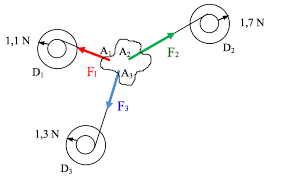
\includegraphics[width=0.24\textwidth]{./img01.png}
\end{wrapfigure}
\subsubsection{Expérience:}

On réalise l'électrolyse d'une solution de chlorure de sodium $(Na^++Cl^-)$.

L'expérience montre qu'il y'a dégagement du dichlore $Cl_2$ au voisinage de l'anode et dégagement du dihydrogène $H_2$ et formation
des ions hydroxydes HOau voisinage de la cathode.


\subsubsection{Interprétation: }

Les espèces chimiques qui existent dans la solution sont : $H_2O$ , $Cl^-$ , $Na^+$ , plus le graphite (qui ne réagit pas) et ses espèces appartiennent aux couples suivants : $Cl_2/Cl^-$
, $Na^+/Na$ , $H_2O/H_2$ et $O_2/H_2O$

\begin{enumerate}
	\item \textbf{Au voisinage de l'anode :} il y'a oxydation : ( C'est le réducteur qui subit l'oxydation)

Parmi les espèces présentes dans l'électrolyseur on a deux réducteurs $H_2O$ et $Cl^-$ appartenant aux couples $Cl_2/Cl^-$ et $O_2/H_2O$

Les oxydations susceptibles de se produire au voisinage de l'anode sont:

(1) \ce{$2Cl^-$ <=> $Cl_{2(g)}$ + $2e^-$}

(2) \ce{$2H_2O$ <=> $O_2$ + $4H^+$ + $4e^-$}


\item \textbf{Au voisinage de la cathode :} il y'a réduction : (C'est l'oxydant qui subit la réduction)

Parmi les espèces présentes dans l'électrolyseur on a deux oxydant $H_2O$ et $Na^+$ appartenant aux couples : $H_2O/H_2$ et $Na^+/Na$

Les oxydations susceptibles de se produire au voisinage de la cathode sont:

(1) \ce{$Na^+$ + $e^-$ <=> $Na$}

(2) \ce{$2H_2O$ + $2e^-$ <=> $H_2$ + $2HO^-$}

(2) \ce{$2H_2O$ <=> $O_2$ + $4H^+$ + $4e^-$}


\item Expérimentalement, on obtient dégagement du dichlore au voisinage l'anode et dégagement du dihydrogène au voisinage de la
cathode.

Donc les réactions qui se produisent effectivement sont:


\item Au voisinage de l'anode : \ce{$2.Cl^-$ <=> $Cl_2$ + $2e^-$}
\item Au voisinage de la cathode : \ce{$2H_2O$ + $2e^-$ <=> $H_2$ + $2HO^-$}

\item L'équation bilan de cette électrolyse est 
\ce{$2H_2O$ + $2Cl^-$ -> $Cl_2$ +  $H_2$ + $2HO^-$}

\end{enumerate}

\begin{tcolorbox}
Conclusion:
\begin{enumerate}
	\item En général dans l'électrolyse, à partir du sens du courant électrique on identifie l'anode et la cathode.

	\item Ensuite à partir des espèces chimiques qui existent dans la cuve à électrolyse, on écrit toutes les oxydations susceptibles de se
produire au voisinage de l'anode et toutes les réductions susceptibles de se produire au voisinage de la cathode(Tout en tenant
compte de l'eau qui est toujours solvant et des électrodes qui peuvent parfois participer à ses réactions),
\item Enfin l'analyse des produits formés permet de connaitre les demi-réactions qui se produisent effectivement à chaque électrode.
\end{enumerate}
\end{tcolorbox}

\subsection{Électrolyse à anode soluble:}
\subsubsection{Intérêt de l’électrolyse à anode soluble:}

\begin{wrapfigure}[1]{r}{0.24\textwidth}
	\vspace{-3.5cm}
	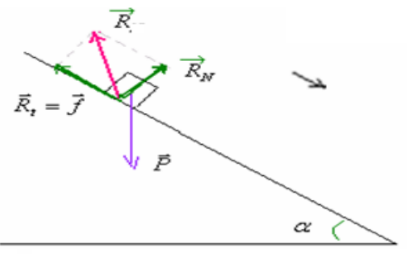
\includegraphics[width=0.24\textwidth]{./img03.png}
\end{wrapfigure}

On rencontre ce type d'électrolyse si l'anode est constituée d'un métal M et la solution électrolytique contient les
ions $M^{m+}$ de ce même métal (qui constitue l'anode).

\begin{enumerate}

	\item Le métal de l'anode s'oxyde selon la demi-équation : \ce{$M_(s)$    <=>  M^{+m} + $m.e^-$}

	\item Le métal M se dépose sur la cathode par réduction des ions 

		$M^{m+}$ selon la demi-équation:
 \ce{ M^{+m} + $m.e^-$  <=> $M_(s)$}

\end{enumerate}





Le bilan de la réaction est nul et cette électrolyse commence à partir de 0V.
L’intérêt de cette électrolyse est le transfert du métal de l'anode vers la cathode ( On l’utilise pour la réalisation de dépôt de
métal sur un support métallique ou pour la purification des métaux).

Chaque fois qu’un atome du métal M disparaît à l’anode, il se forme un atome du métal M sur la cathode : la masse
du métal déposée sur la cathode est égale à celle perdue par l’anode.
Chaque fois qu’un ion $M^{m+}$ disparaît à la cathode, il se forme un ion $M^{m+}$ à l’anode ,le nombre d’ions $M^{m+}$ reste
constant dans la solution qui de ce fait la solution conserve sa teinte.



\subsubsection{Exemple d'électrolyse à anode soluble:}
\begin{wrapfigure}[3]{r}{0.24\textwidth}
	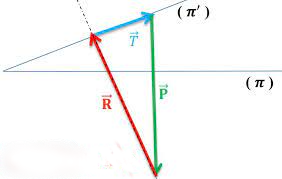
\includegraphics[width=0.24\textwidth]{./img04.png}
\end{wrapfigure}
utilisant une anode en cuivre Cu ( la cathode est une clef en fer Fe) .


On obtient un dépôt de cuivre sur la clef. et on constate la diminution de l'anode. C'est une électrolyse à anode soluble. 



bilan de l'électrolyse : transfert du cuivre de l'anode vers la cathode.


\section{Applications de l'électrolyse}

Malgré le coût élevé de l'énergie électrique consommée ,l'électrolyse a de nombreuses applications industrielles comme:

\begin{enumerate}
	\item La préparation et la purification de nombreux métaux comme l'aluminium,le zinc,le cuivre, l'argent et d'aures métaux.
	\item La préparation d'eau oxygénée ou du dichlore ou du dihydrogène,...
\item La protection avec une couche d’or ou d’argent ou par d’autres métaux qui se dépose à la surface de divers objets pour
améliorer leurs aspects.
\item La recharge des accumulateurs des voitures ou de téléphone sont des applications courantes de l'électrolyse.
Un accumulateur peut fonctionner spontanément comme générateur ( tout en jouant le role d'une pile) et aussi en sens inverse
pour se recharger , car quand on le branche aux bornes d'un générateur qui impose un sens de courant inverse il se charge.
Prenons comme exemple l'accumulateur de plomb (batterie d’automobile). :il est constitué de deux électrodes en plomb dont
l'une est recouverte de dioxide de plomb plongeant dans une solution d'acide sulfirique et de sulfate de plomb.



\end{enumerate}
La force électromotrice est de l'ordre de 2V , dans une batterie de voiture elle est égale à 12 V car on en associe six en serie.









%\begin{figure}[h!]
	%\begin{center}
	%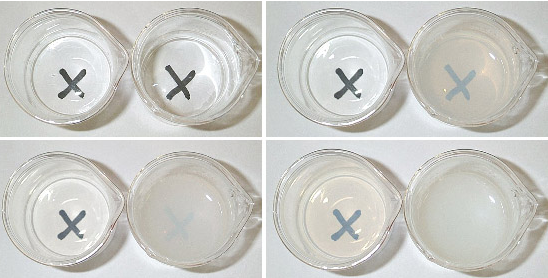
\includegraphics[width=0.5\textwidth]{./img/TRLconcentration.png}
%\end{center}
%\vspace{-1cm}
%\end{figure}



%\begin{wrapfigure}[10]{r}{0.5\textwidth}
%    \includegraphics[width=0.5\textwidth]{./img/img00.png}
%\end{wrapfigure}


%\begin{center}
   %\begin{tabular}{|c|c|c|}
      %\hline
      %Indicateur coloré & Couleur de l’espèce acide & Couleur de l’espèce base\\\hline
      %BBT               & Jaune                     & Bleue\\\hline
      %Hélianthine       &Rose                       & Jaune\\\hline
      %Phénolphtaléine   & inclore                   & rose \\\hline
   %\end{tabular}
%\end{center}

\end{document}

